%% all about growing, placing, imaging, filtering carbon nanotubes

\chapter{Carbon Nanotube Growth and Placement}
\label{sec:growth}
\chaptermark{Growth and Placement}

There are several methods that can be used to deposit nanotubes onto a substrate. Two of these methods, random dispersion and catalyst island growth, are discussed here. Additional methods, such as stamping \cite{Wu2010, Pei2012}, were not utilized for this work and will not be discussed.

\section{Random Dispersion}

The oldest, and least reliable, method of nanotube device fabrication, is what will be referred to as random dispersion. First, nanotubes are grown in bulk through chemical vapor deposition (or other preferred method). Then, the nanotubes are suspended in a solution. Finally, the nanotubes are cast onto a substrate. Nanotubes can then be located relative to some predefined markers on the substrate.

\subsection{Catalyst}
\label{subsec:disperse_catalyst}

All of the devices discussed in this thesis have utilized the same, iron-based catalyst \cite{Kong1998, Kong1998a}. The simplest way to create this catalyst is to combine the ingredients in Table \ref{table:powder_catalyst} in a mortar and pestle and grind until it turns a uniform dark orange color. Adding some additional alumina seems to promote growth of longer tubes, possibly by lowering the density of tubes grown from each alumina/iron/molybdenum particle.

\begin{table}
	\centering
	\caption{Powder Catalyst}
    \begin{tabular}{ c | c }
    	\hline
        \ce{Fe(NO3)3*9H2O} & \SI{20}{\milli\gram} \\ \hline
        \ce{MoO2(acac)2} & \SI{5}{\milli\gram} \\ \hline
        \ce{Al2O3} & \SI{15}{\milli\gram} \\ \hline
    \end{tabular}
    \label{table:powder_catalyst}
\end{table}

\subsection{Growth}
\label{subsubsec:powder_cvd}

Of the many possible techniques for nanotube growth, we choose chemical vapor deposition for its simple implementation. The process is carried out in a Lindberg Blue tube furnace using a 1 inch diameter quartz tube. The furnace, quartz tube, and exhaust filtering are seen in Figure~\ref{fig:furnace_setup}. Despite its poor looks, this setup has been repeatedly, and successfully, leak checked. Oxygen leaks can be detrimental to the nanotube growth process by forming \ce{CO} and \ce{CO2} with any free carbon.

\begin{figure}
    \centering
    \includegraphics[width = 0.8\textwidth]{chapter3/furnace_setup.jpg}
    \caption{The tube furnace fitted with a 1" diameter quartz tube. The tube is sealed at both ends using 1" rubber tubing, cable clamps, and KF25 fittings. Gas flows from left to right in the picture. The gas flows out of the furnace into a mineral oil bubbler to keep hot hydrogen from reaching the air in the room. Gas then flows from the bubbler into the building exhaust.}
    \label{fig:furnace_setup}
\end{figure}

The gases used in the CVD process, argon, hydrogen, and methane, are fed into the furnace using a custom-made gas handling panel. This was originally constructed by Matt Oresky, a JHU undergraduate working in our lab with post-doc Atikur Rahman. The panel has three gas channels, each with its own analog flowmeter, needle valve, and on/off valve. A digital flowmeter placed at the right side of the panel reads the total flow of combined gas exiting the panel to the furnace. The gas handling panel can be see in Figure~\ref{fig:gas_panel}

\begin{figure}
    \centering
    \includegraphics[width = 0.8\textwidth]{chapter3/gas_panel.jpg}
    \caption{The gas handling panel for our Lindberg tube furnace. Gas flow is from left to right.}
    \label{fig:gas_panel}
\end{figure}

The growth procedure begins with filling a ceramic crucible with the iron catalyst described in \ref{subsec:disperse_catalyst}. The catalyst should be spread in a thin layer across the bottom of the crucible, which is then loaded into the center of a 2-4 foot long quartz tube. The tube is sealed at each end, one side connected to the gas handling panel, and the other connected to the mineral oil filter and building exhaust. Our standard nanotube growth recipe is as follows: 

%can i remove the spacing from between these list items?
\begin{enumerate}
	\item Purge the tube by flowing \SI{2000}{\sccm} of Ar for 20 minutes
	\item Heat tube to \SI{1000}{\degreeCelsius} while flowing \SI{1000}{\sccm} Ar and \SI{200}{\sccm} \ce{H2}
	\item Flow \SI{2000}{\sccm} \ce{CH4} and \SI{200}{\sccm} \ce{H2} for 10 minutes.
	\item Set temperature to \SI{0}{\degreeCelsius} and let the furnace cool while flowing \SI{1000}{\sccm} Ar and \SI{200}{\sccm} \ce{H2}
\end{enumerate}

\noindent The actual nanotube growth occurs during the methane flow step. The \SI{200}{\sccm} \ce{H2} flow can be omitted, but it does seem to help promote nanotube growth. The flow rates do not need to be precise. Most nanotubes grow in the first few seconds of methane flow regardless of the flow rate. The Ar and \ce{H2} are simply to keep \ce{O2} and \ce{H2O} out of the tube. 

\subsection{Nanotube Placement}

After the CVD process, the nanotubes remain attached to the iron\slash alumina\slash molybdenum catalyst particles, which must be removed before depositing onto a silicon substrate. The nanotube\slash catalyst powder is first scraped from the ceramic crucible used in the tube furnace. The powder is then mixed with either dichloroethane or dichlorobenzne in a \SI{1}{\milli\gram} to \SI{10}{\milli\liter} ratio. Dichlorobenze has been found to leave less residue after deposition, but may promote more damage to nanotubes during sonication. Some attempts were made to use water along with the surfactant SDS. However, SDS turned out to be difficult to remove and no devices were made in this way.

To remove the catalyst particles from the nanotubes, the solution described above must be placed in an ultrasonic bath for 1-60 minutes. The amount of time needed varied a great deal depending on the equipment and solvent used. The goal of this step is to break up large pieces of catalyst, separate nanotube bundles, and break individual nanotubes away from their catalyst particles. Sonication can be stopped when no large pieces of catalyst\slash nanotube material are visible and the solution has a uniform black color. Leaving the solution in the sonicator for too much time will begin to break long nanotubes. 

When sonication is complete, the solution is transferred to a centrifuge. This step is intended to precipitate the loose catalyst particles from the solution, while leaving the much lighter nanotubes suspended. The centrifuge used in our lab runs at \SI{2200}{\rpm} and nanotube solutions are left inside for 5-10 minutes. Once the centrifuge stops, the precipitate is discarded and the supernate, containing the suspended nanotubes, is reserved. We also tested using a high-speed, air-powered centrifuge running at \SI{100000}{\rpm} to separate nanotubes and catalyst. This did lead to much better catalyst separation and cleaner results,.

Now the solution is ready for deposition on a silicon substrate. The substrates are typically pre-patterned with a set of reference markers placed by optical (\ref{subsec:optical}) or electron beam lithography (\ref{sec:ebeam_lith}). An example of a patterned substrate can be seen in Figure \ref{fig:markers}

\begin{figure}
    \centering
    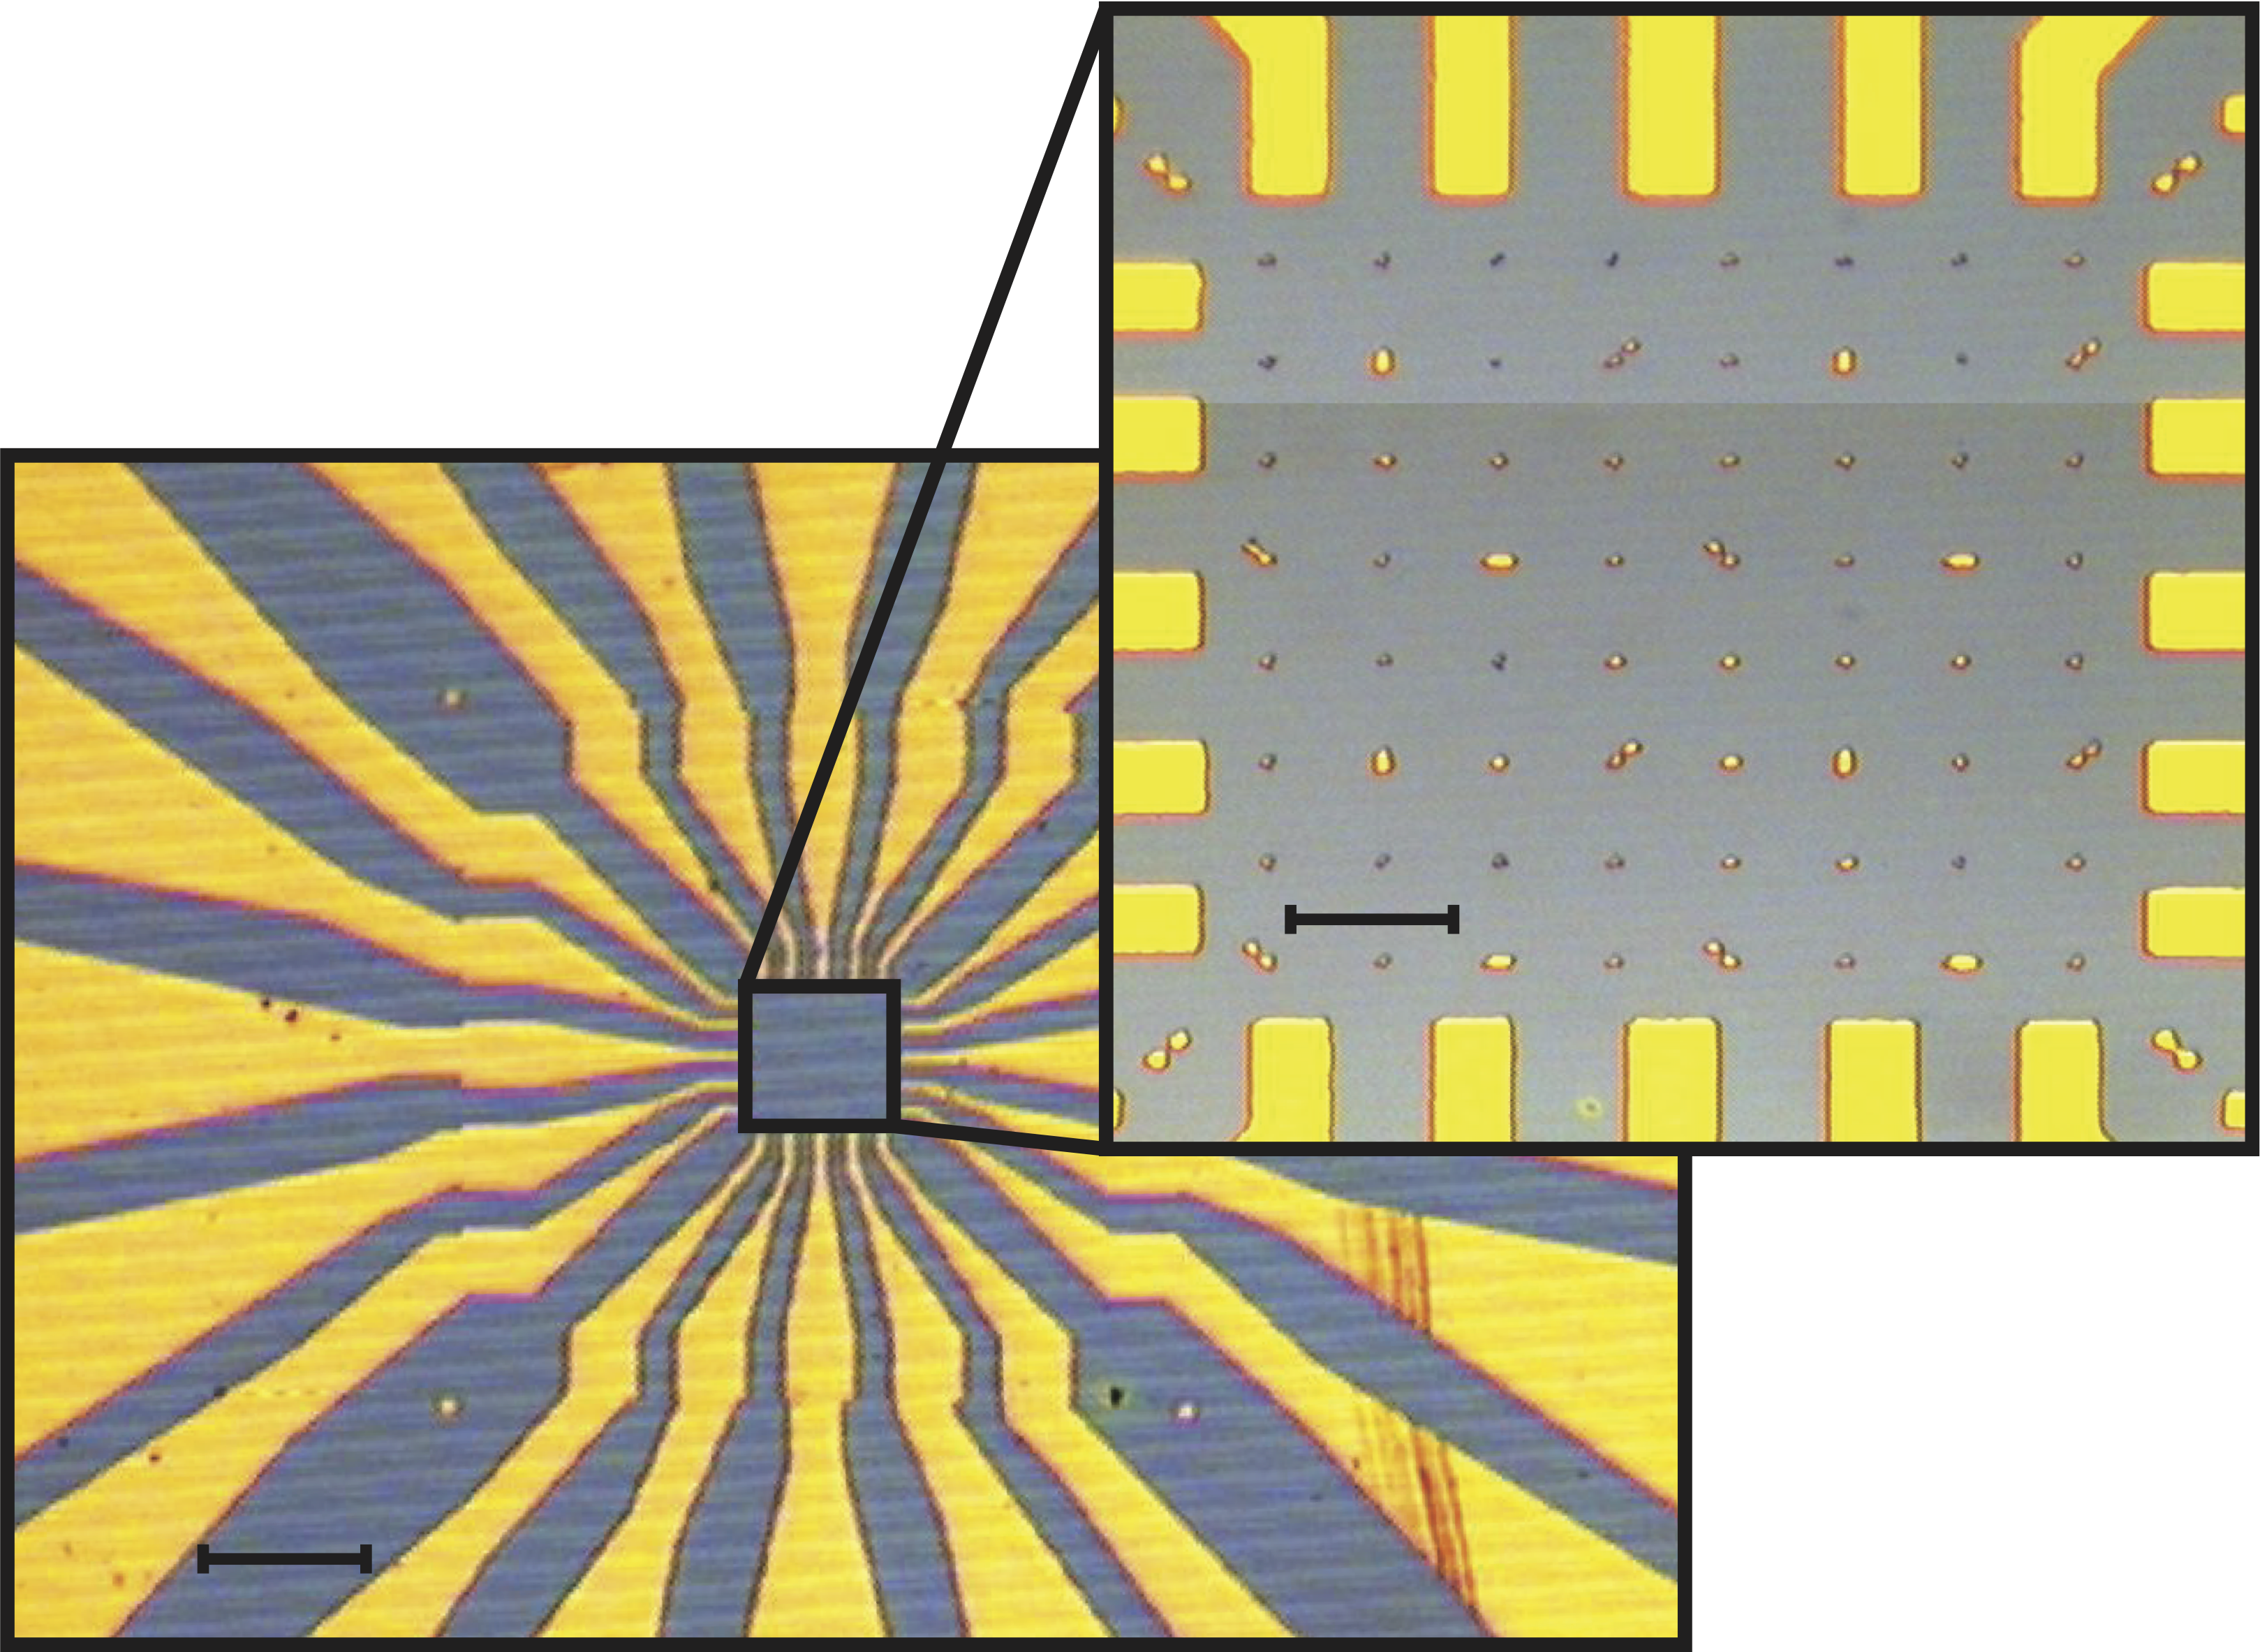
\includegraphics[width = 0.8\textwidth]{chapter3/markers.eps}
    \caption{A \ce{Si}/\ce{SiO2} substrate with \SI{1}{\micro\meter} \ce{Au} markers. Left scale bar: \SI{100}{\micro\meter}. Right scale bar: \SI{20}{\micro\meter} }
    \label{fig:markers}
\end{figure}

\subsection{Conclusion}

Despite having some success fabricating devices using randomly dispersed nanotubes and EFM scans, the process was found to be too unreliable for frequent use. The main failure point was the preparation of nanotube solutions after growth. The concentrations varied significantly, often producing samples with dense nanotube coverage or no nanotubes found in the regions imaged. Additionally, the process of making a suspended nanotube solution is time consuming. Even those solutions with a useful concentration of nanotubes only remain fully suspended for less than 1 hour.

\section{Catalyst Island Growth}
\label{subsec:catalyst_island}

In 1998 \cite{Kong1998a}, it was discovered that the same type of catalyst used to grow nanotubes in powder form (Section \ref{subsec:disperse_catalyst}), could be suspended in solution, patterned, and used to grow nanotubes directly on silicon substrates. When paired with high melting point metals and optical lithography, nanotubes can be grown directly on patterned substrates in known locations. Devices prepared this way take just a fraction of the time to produce. 

\subsection{Catalyst} 

Many different types of catalyst particles can be used in the growth of carbon nanotubes. The ideal catalyst for patterned growth must be compatible with electron beam or optical lithography. Table \ref{table:catalysts} lists most of the catalysts tested in the Markovic lab. To test each catalyst, sputtered molybdenum leads were patterned using the mask aligner and Futurex NR9 resist. Catalyst islands were then patterned using electron beam lithography. Figure \ref{fig:catalyst_islands} shows an example of a substrate with Mo leads and catalyst islands.

\begin{figure}
	\centering
	\includegraphics[width = 0.8\textwidth]{chapter3/catalyst_island.eps}
	\caption{A \ce{Si}/\ce{SiO2} substrate with \SI{3}{\micro\meter} catalyst islands and \ce{Mo} leads. Left scale bar: \SI{100}{\micro\meter}. Right scale bar: \SI{20}{\micro\meter} }
	\label{fig:catalyst_islands}
\end{figure}

\begin{table}
	\centering
	\caption{Patterned Catalysts}
    \begin{tabular}{| r | c || p{70mm} |}
    	\hline
    	\textbf{Catalyst} & \textbf{Suspended In} & \textbf{Results} \\ \hline
        Fe/Mo/alumina \cite{Kong1998} & Methanol & Easy to pattern. Liftoff difficult. Slowly attacks PMMA mask. Appeared to promote to gate leaks through the \ce{SiO2} layer. \\ \hline
        Fe/Mo/alumina \cite{Aurich2012} & IPA & Poor adhesion to substrate. \\ \hline
        Fe/Mo/alumina \cite{Ouellette2008} & DI water & Easy to pattern. Excellent adhesion. No gate leak problems. \\ \hline
        \ce{FeCl3} \cite{Hong2005} & DI water & Excellent adhesion to substrate. Not compatible with PMMA mask. Left substrate entirely covered in catalyst. May work well with PDMS stamp. \\ \hline
        thermally evaporated Fe \cite{Biercuk2004, Kang2007} & None & Very easy to pattern. Liftoff is clean. Difficult to control the thickness below \SI{1}{\nano\meter} as required. \\ \hline
    \end{tabular}
    \label{table:catalysts}
\end{table}

All of the devices discussed in this thesis were produced using the Fe\slash Mo\slash alumina catalyst suspended in water. The islands were patterned using electron beam lithography. Catalyst is deposited in the following way:

\begin{enumerate}
	\item Add the powder catalyst from Table \ref{table:powder_catalyst} to \SI{15}{\milli\liter} of DI water and stir for 12 hours
	\item Sonicate the solution for 30 minutes
	\item Cover the sample in catalyst solution for 30 minutes
	\item Dry with \ce{N2} gun
	\item Liftoff by sonicating in acetone for 5 minutes, soaking in a clean acetone for 5 minutes, followed by an isopropanol rinse for 1 minute and a DI water rinse for 1 minute
\end{enumerate}

Depositing the catalyst islands in a reproducible way proved to be the most difficult step in the fabrication of nanotube samples. It is suspected that baking the catalyst on a hot plate to dry the solution leads directly to gate leaks in the \ce{SiO2} layers and later device failure. Thus, there is no baking step in the deposition of our catalyst islands.

\subsection{Growth}
\label{subsubsec:substrate_cvd}

The recipe for on-substrate growth of nanotubes used in this thesis is very similar to the growth recipe for powder catalyst discussed in Section \ref{subsubsec:powder_cvd}. This recipe was developed over the course of several years from many points of reference \cite{Kong1998, Kong1998a, Dirks2010, Huang2003, Huang2004, Zhang2013, Hong2005} and a my own notes. The recipe is optimized for the 1 inch Lindberg tube furnace as seen in Figures \ref{fig:furnace_setup} and \ref{fig:gas_panel}. Most samples are placed in a smaller \SI{1}{\centi\meter} diameter, 1 foot long quartz tube, then placed in the larger 1 inch diameter quartz tube. This was done to make the samples easier to load into the 1" tube, as well as to reduce turbulence in the gas flow across the sample \cite{Hong2005}. 

The standard nanotube growth recipe used in this work is below:

\begin{enumerate}
	\item Purge the tube by flowing \SI{2000}{\sccm} of Ar for 20 minutes
	\item Heat the tube to \SI{250}{\degreeCelsius} while flowing \SI{300}{\sccm} Ar and \SI{150}{\sccm} \ce{H2}
	\item Wait for at least 1 hour
	\item Heat the tube to \SI{700}{\degreeCelsius} while flowing \SI{300}{\sccm} Ar and \SI{150}{\sccm} \ce{H2}
	\item Wait for 10 minutes
	\item Heat tube to \SI{950}{\degreeCelsius} while flowing \SI{300}{\sccm} Ar and \SI{150}{\sccm} \ce{H2}
	\item Wait for the temperature to stabilize
	\item Flow \SI{700}{\sccm} \ce{CH4} and \SI{150}{\sccm} \ce{H2} for 10-15 minutes
	\item Set temperature to \SI{0}{\degreeCelsius} and let the furnace cool while flowing \SI{300}{\sccm} Ar and \SI{150}{\sccm} \ce{H2}
\end{enumerate}

In almost every case this recipe has grown nanotubes successfully. Steps 2 and 3 are included to remove water vapor from the air that might have collected inside the quartz tube on humid days \cite{Dirks2010}. Steps 4 and 5 are meant to remove iron oxide from the iron nanoparticles that make up the catalyst. 

The most common point of failure has been related to the patterned molybdenum leads on the substrate. Molybdenum oxidizes rapidly at high temperatures. Therefore, any oxygen contamination in the tube during the growth process will form a \ce{MoO} layer that is then quickly removed by reacting with the high temperature \ce{H2} flow. This process repeats and can lead to the Mo leads being entirely etched away. Additionally, it has been found that opening the furnace too soon during cooling can lead to the Mo leads peeling off of the substrate. This appears to be caused by some super-heating due to IR radiation reflecting off of the surfaces of the sample and quartz tube. It is a strange phenomenon that is avoided by allowing the furnace to cool to less than \SI{300}{\degreeCelsius} before opening the lid. These problems could also be solved by using a different high temperature metal such as a W/Pt bilayer, common in many other nanotube projects. Molybdenum was chosen for this work because it is easy to sputter and much more affordable.

\subsection{Conclusion}

Growing nanotubes from catalyst islands near predefined leads and markers offers a huge improvement over the method of random dispersion. Nanotubes produced with this method are longer, cleaner, and easier to locate. These improvements, along with the ability to produce many more samples in much less time, made this method the obvious choice for device fabrication.

\section{Imaging Nanotubes}
\label{subsubsec:imaging_disperse}

Nanotubes on a \ce{SiO2} surface can be located in a number of ways. This section will review a number of different methods, focusing on improvements made in the course of this thesis work.

\subsection{Atomic Force Microscopy}

With nanotubes that have been drop cast onto the surface, the standard method is to locate the tubes relative to the predefined markers using a tapping mode atomic force microscope (AFM). An example of an image created this way is seen in Figure \ref{fig:cnt_au_markers}. 

\begin{figure}
	\centering
	\includegraphics[width = 0.8\textwidth]{chapter3/cnt_au_markers.eps}
	\caption{A composite image made from several AFM height measurements of a sample with nanotubes dispersed over a  substrate with \SI{1.5}{\micro\meter} gold markers. The scale bar is \SI{10}{\micro\meter}.}
	\label{fig:cnt_au_markers}
\end{figure}

This method is very reliable, but extremely time consuming. In order to resolve nanotubes, as well as the predefined markers in the image, AFM scan sizes must be limited to \SI{25}{\square\micro\meter}. Each of these scans takes 30 minutes and many scans are needed to fully image one patterned substrate. Looking closely at Figure \ref{fig:cnt_au_markers}, there are 12 scans covering less than half the substrate. Due to vibrational noise and piezo limits, some images are slightly warped. Stitching the images together is time consuming and inaccurate.

\subsection{Electric Force Microscopy}

The Digital Instruments Nanoscope 3 used in our lab is also capable of making electric force microscope (EFM) measurements. An EFM image is made by first measuring the height across the sample in standard tapping mode, then using that height data to run a second 'interleave' scan at a fixed height with a bias voltage applied between the tip and sample. By holding the tip at a fixed height, van der Waals interactions between the tip and sample are constant and the only force measured is the electrostatic force from the applied bias voltage. Contrast in the resulting images is related to the different conductivities of the objects on the sample \cite{Bockrath2002}. Thus, conducting (and semiconducting) nanotubes have a high contrast against the insulating \ce{SiO2} substrate. An example of this type of image is shown in Figure \ref{fig:cnt_efm}

\begin{figure}
	\centering
	\includegraphics[width = 0.8\textwidth]{chapter3/cnt_efm.eps}
	\caption{An EFM image of nanotubes dispersed over a substrate with \SI{1.5}{\micro\meter} gold markers. The markers have been automatically located using the height data and highlighted in blue on the EFM image. The scale bar is \SI{10}{\micro\meter}.}
	\label{fig:cnt_efm}
\end{figure}

An entire patterned substrate can be scanned using this method in about 1 hour. The scan size can be increased up to \SI{75}{\square\micro\meter} due to the false contrast provided by the large electrostatic forces between the nanotubes and the tip. Rather than appearing as \SI{1}{\nano\meter} in diameter, the tubes appear in the EFM image to be about 100 times their real diameter. This was a notable improvement over locating nanotubes using AFM height scans alone. Comparing Figure \ref{fig:cnt_au_markers} and Figure \ref{fig:cnt_efm}, it is clear the EFM image is far more useful in locating nanotubes.

\subsection{EFM Through PMMA}

All of the same techniques from Section \ref{subsubsec:imaging_disperse} can be applied to imaging nanotubes grown from patterned catalyst islands. However, because the substrates are not covered in closely spaced markers, it was found that tapping mode AFM height scans were not useful. Scans could only cover a small part of the sample and the resulting images were difficult to orient.

Using electric force microscopy (EFM) made it possible to scan the entire region of interest on the sample in one measurement. An example of this type of scan is shown in Figure \ref{fig:efm_islands}a. As can be seen in that figure, it was difficult for the AFM tip to avoid crashing into the catalyst islands during the EFM sweep. The catalyst islands are several hundred nanometers in height while the other features on the substrate are less than \SI{10}{\nano\meter}. Such height differences make large area scans difficult in tapping mode. This problem can be avoided by coating the sample in PMMA before scanning with the EFM, as seen in Figure \ref{fig:efm_islands}b. The PMMA coating smooths the height differences between the substrate and catalyst islands, without compromising the contrast between the insulating substrate and conducting nanotubes. The idea was adopted from a 2007 paper in which the authors attempted to locate nanotubes suspended in a PMMA layer in three dimensions \cite{Jespersen2007}.

\begin{figure}
	\centering
	\includegraphics[width = 1.0\textwidth]{chapter3/efm_islands.eps}
	\caption{(a) Frequency data collected from an EFM scan of a catalyst island sample after nanotube growth. (b) Frequency data collected from an EFM scan of a similar sample. Prior to the scan this sample was coated with a \SI{250}{\nano\meter} PMMA layer. Both scale bars are \SI{10}{\micro\meter}. }
	\label{fig:efm_islands}
\end{figure}

\subsection{Scanning Electron Microscopy}

In 2002, a paper \cite{Brintlinger2002} was published illustrating that a scanning electron microscope (SEM), operating at a low accelerating potential could provide a similar type of false contrast image as produced by the EFM. The insulating substrate tends to collect charge from the electron beam, while the conducting nanotubes do not. This produces an image in which the nanotubes appear as bright lines about 100 times their actual diameter. An example of this is seen in Figure \ref{fig:sem_islands}. 

\begin{figure}
	\centering
	\includegraphics[width = 0.8\textwidth]{chapter3/sem_islands.eps}
	\caption{A scanning electron micrograph of a catalyst island sample after nanotube growth. The scale bar is \SI{10}{\micro\meter}.}
	\label{fig:sem_islands}
\end{figure}

Typically, an EFM scan of a sample will take 45 minutes. A SEM image of the same sample takes less than 2 minutes. However, the SEM can introduce some carbon contamination from the high energy electrons passing through small amounts of oil mist back-streaming into the vacuum chamber from the mechanical roughing pump. Due to the large number of samples that were produced to obtain the data in this thesis, it was decided that contamination from the SEM was an acceptable risk, given the immense time savings.

\section{Image Filtering}

Once it became clear that the scanning electron microscope was by far the most efficient and reliable way to locate carbon nanotubes on a substrate, it also became important to optimize those images to revel the most information possible. The resolution and contrast in the SEM images produced in our lab are limited due the the use of a thermionic \ce{LaB6} filament. Unlike field emission scanning electron microscopes, which are more common in nanofabrication, the thermionic scanning electron microscope has a large initial crossover size, requiring more electromagntic lens focusing to produce a sufficiently small beam size for imaging. This problem is exasperated when using low accelerating potentials (500-\SI{3000}{\volt}), which are crucial to achieving good contrast of carbon nanotubes on a silicon substrate.

\subsection{Histogram Equalization}

This method was based on two corrections. First, a plane fit to correct for the position of the secondary electron detector. Second, finding the histogram of all o

\subsection{Matched Filter Bank}

Matched filter banks are a well known technique that have been used very successfully to filter retinal images in medicine \cite{Chaudhuri1989}. This technique has previously been adapted to high resolution images of SEM bundles \cite{Guerrero2014}. The following section describes the implementation of this method to filter images of single walled carbon nanotubes grown on insulating substrates. 
%% nanotube profiles -> kernel -> filtering/thresholding

\subsubsection{Nanotube Profile Model}

To begin building the matched filter bank, the profile shape of a single nanotube from the SEM image must be determined. To find this shape, a random set of 25 SEM images was selected. From each of these images, two nanotubes were chosen. Those nanobues can be seen in Figure (...)a. Each of these images was then rotate such that the longest, straight portion that could be identified by eye was oriented vertically. The profile of the nanotube was averaged over that long straight section. These results are plotted in ...

% figures I want for this section...
% 1. original data set
% 2. extracted profiles with fits, histograms of k, L data
% 3. filter bank, each filter applied, original image, result

Based on the shape of these profiles a truncated sinc function was chose to fit the nanotube profile. 

%% equation for sinc function including truncated region

This fuction was chosen because it captures the dark regions beside the nanotube, while still only requiring one fit parameter.

\subsubsection{Filter Kernel}

\subsubsection{Results}